\documentclass[8pt]{article} %{report}
\usepackage{fullpage}
\usepackage{graphicx}
\usepackage{subfigure}
\usepackage{float}
\usepackage[mathletters]{ucs}
\usepackage[utf8x]{inputenc}
\usepackage{multirow}
\usepackage{hyperref}
\usepackage{wrapfig}
\usepackage{tabto}
\usepackage{listings}
\usepackage{color,soul}
\usepackage{subcaption}
\usepackage{amsmath}

\definecolor{dkgreen}{rgb}{0,0.6,0}
\definecolor{gray}{rgb}{0.5,0.5,0.5}
\definecolor{mauve}{rgb}{0.58,0,0.82}
\lstset{frame=tb,
  language=MATLAB,
  aboveskip=3mm,
  belowskip=3mm,
  showstringspaces=false,
  columns=flexible,
  basicstyle={\small\ttfamily},
  numbers=none,
  numberstyle=\tiny\color{gray},
  keywordstyle=\color{blue},
  commentstyle=\color{dkgreen},
  stringstyle=\color{mauve},
  breaklines=true,
  breakatwhitespace=true,
  tabsize=3}

\begin{document}

\begin{titlepage}
    \begin{center}
        
        \vspace*{1cm}
            
        \Huge
        \textbf{Department Of Aerospace Engineering , IIT Madras}
	
        \vspace{0.5cm}

	
\includegraphics[width=0.4\textwidth]{IITM_logo.png}

        \LARGE
        AS6320: Acoustic Instabilities in Aerospace Propulsion \\
	\vspace{2cm}
	An Exact Solution for 1D Acoustic Fields in Ducts with an Axial Temperature Gradient
            
        \vspace{1.5cm}
            
        \textbf{AE21B002\\Abhigyan Roy\\}
            
        \vfill
           
        \vspace{0.8cm}
            
        \Large
        Sunday\\
        March 31, 2024\\
            
    \end{center}
\end{titlepage}

\newpage
\tableofcontents
\vspace{2cm}
\listoffigures

\counterwithin{equation}{section}

\newpage

\section{Abstract}
This study focuses on numerically solving the one-dimensional wave equation in ducts with axial temperature gradients. The second-order ODE is transformed into a system of first-order ODEs, suitable for solving with numerical methods like Runge Kutta. The results are confirmed using this paper as reference.\cite{refpaper}%This approach allows for understanding wave propagation in practical systems, crucial for engineering design and analysis.

\section{Introduction}

The study of one-dimensional acoustic fields within ducts featuring a mean temperature gradient is of significant scientific and practical importance. This problem impacts various engineering applications, such as understanding the influence of axial temperature gradients on sound wave propagation, stability analysis of disturbances in ducts, and design considerations for combustion and thermal systems. Obtaining exact analytical solutions for such wave systems in ducts with temperature gradients is crucial for these endeavors.\\\\
\begin{figure}[H]
    \centering
    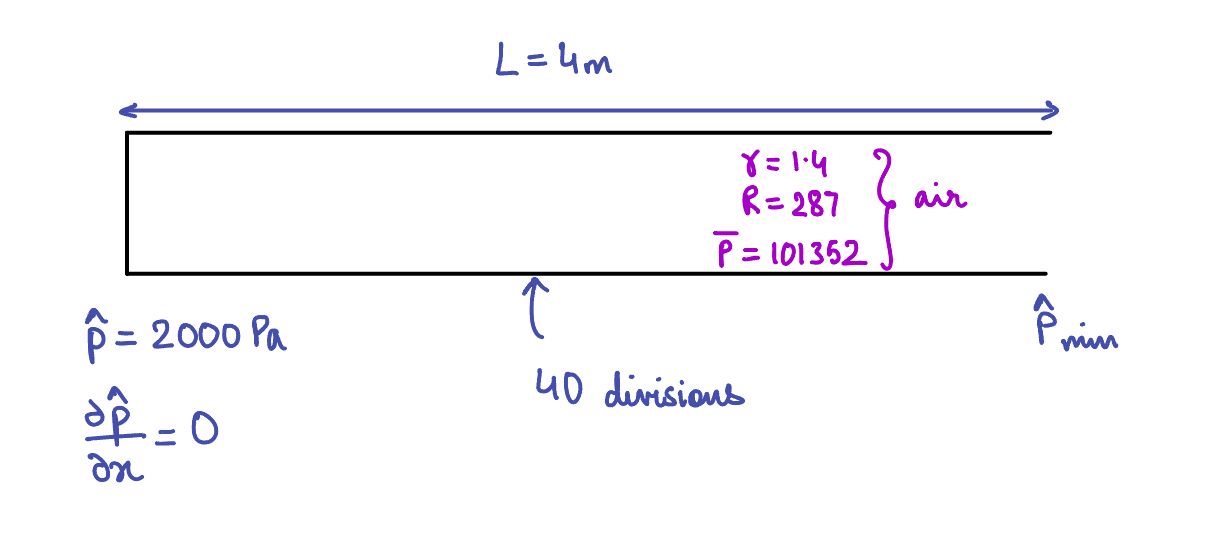
\includegraphics[width=0.6\linewidth]{setup.jpg}
    \caption{Physical Setup}
    \label{fig:setup}
\end{figure}
In this study, a numerical solution method for one-dimensional wave behavior in a duct as shown in the figure above with arbitrary axial temperature profiles and boundary conditions is outlined. The procedure involves deriving the wave equation for a constant area duct with the temperature gradient, reducing it to a second-order ordinary differential equation, and transforming it into a standard system of differential equations dependent on the mean temperature. This allows for obtaining numerical solutions for various temperature profiles.\\\\
It should be noted that the analysis in this study does not consider the effects of mean flow, limiting its applicability to scenarios with Mach numbers less than a certain threshold. This analytical framework provides a valuable tool for understanding and designing systems involving one-dimensional acoustic oscillations in ducts with temperature gradients.


\section{Derivation of Wave Equation}
We start with the assumptiosn that the gas/medium is perfect, inviscid and non-heat conducting. 
The \textbf{momentum} equation in one dimension is,
\begin{equation}
\rho \frac{\partial u}{\partial t} + \rho u \frac{\partial u}{\partial x} + \frac{\partial p}{\partial x} = 0
\end{equation}\label{eq:3.1}
The \textbf{energy} equation in one dimension is,
\begin{equation}
\frac{\partial p}{\partial t} + u \frac{\partial p}{\partial x} + \gamma p \frac{\partial u}{\partial x} = 0
\end{equation}\label{eq:3.2}
The \textbf{equation of state} is
\begin{equation}
p = \rho R T
\end{equation}\label{eq:3.3}
Expressing each of the dependent variables as the sums of steady and time dependent, small amplitude solutions as such\\\\
u = $\bar{u}$(x) + u'(x,t); $\quad\quad$   p = $\bar{p}$(x) + p'(x,t); $\quad\quad$   $\rho$ = $\bar{\rho}$(x) + $\rho$'(x,t); $\quad\quad$ T = $\bar{T}$(x) + T'(x,t); \\
we substitute it in the above equations.\\
The mean pressure $\bar{p}$ in the duct is constant, as demonstrated by the steady momentum equation's solution, provided that the mean flow Mach number is less than 0.1.\\\\
From equation 3.1, we get $\quad$ $\rho \frac{\partial [\bar{u} + u'] }{\partial t} + [\bar{\rho} + \rho']  [\bar{u} + u'] \frac{\partial [\bar{u} + u'] }{\partial x} + \frac{\partial [\bar{p} + p'] }{\partial x} = 0 $\\ which becomes the following on substituting for steady state as well as considering the variable fluctuations are small, \textbf{linearised momentum equation}
\begin{equation}
\frac{\partial u'}{\partial t} + \frac{1}{\bar{\rho}} \frac{\partial p'}{\partial x} = 0
\end{equation}\\
From equation 3.2, we get $\quad$ $\frac{\partial [\bar{p} + p']}{\partial t} + [\bar{u} + u'] \frac{\partial [\bar{p} + p']}{\partial x} + \gamma [\bar{p} + p'] \frac{\partial [\bar{u} + u']}{\partial x} = 0$\\
which becomes the following on substituting for steady state as well as considering the variable fluctuations are small, \textbf{linearised energy equation}
\begin{equation}
\frac{\partial p'}{\partial t} + \gamma \bar{p} \frac{\partial u'}{\partial x} = 0
\end{equation}\\
From equation 3.3, we get $\quad$ $[\bar{p} + p'] = [\bar{\rho} + \rho'] R [\bar{T} + T']$\\
which becomes the following on substituting for steady state as well as considering the variable fluctuations are small 
\begin{equation}
p' = \bar{\rho} R T' + \rho' R \bar{T}
\end{equation}\\
The steady state equation of state is $\bar{p} = \bar{\rho} R \bar{T}$\\
We assume that $\bar{p}$ is constant in the duct, so its derivative is zero. Thus, taking derivating of steady state equation of state, we get the relation\\
\begin{equation}
\frac{1}{\bar{T}}\frac{\partial \bar{T}}{\partial x} + \frac{1}{\bar{\rho}}\frac{\partial \bar{\rho}}{\partial x} = 0
\end{equation}\\\\
Taking the spatial derivative of equation 3.4 and time derivative of equation 3.5, we get\\
$\frac{\partial^2 u'}{\partial t \partial x} + \frac{1}{\bar{\rho}} \frac{\partial^2 p'}{\partial x^2} - \frac{1}{\bar{\rho}^2} \frac{\partial \bar{\rho}}{\partial x} \frac{\partial p'}{\partial x} = 0$ $\quad\quad$ and $\quad\quad$  $\frac{\partial^2 p'}{\partial t^2} + \gamma \bar{p}  \frac{\partial^2 u'}{\partial x \partial t} = 0$\\\\
Multiplying the first equation by $\bar{\rho}$, and dividing the second equation by $\gamma \bar{p}$ and then subtracting them, we get\\\\
$\frac{\partial^2 p'}{\partial x^2} - \frac{1}{\bar{\rho}} \frac{\partial \bar{\rho}}{\partial x} \frac{\partial p'}{\partial x} - \frac{\bar{\rho}}{\gamma \bar{p} } \frac{\partial^2 p'}{\partial t^2} = 0$ \\\\
We substitute for $\frac{1}{ \bar{\rho}}\frac{\partial \bar{\rho}}{\partial x}$ using equation 3.7, and finally get the wave equation with a temperature gradient as
\begin{equation}
\frac{\partial^2 p'}{\partial x^2} + \frac{1}{\bar{T}} \frac{\partial \bar{T}}{\partial x} \frac{\partial p'}{\partial x} - \frac{\bar{\rho}}{\gamma \bar{p} } \frac{\partial^2 p'}{\partial t^2} = 0
\end{equation}
Assuming that the solution has a periodic time dependence, we subsitute for p'(x,t) = $\hat{p} e^{- i \omega t}$
\begin{equation}
\frac{\partial^2 \hat{p}}{\partial x^2} + \frac{1}{\bar{T}} \frac{\partial \bar{T}}{\partial x} \frac{\partial \hat{p}}{\partial x} + \frac{\omega^2 \bar{\rho}}{\gamma \bar{p} } \hat{p} = 0
\end{equation}\label{eq:3.9}
We assume that the temperature variation is linear in the form of
\begin{equation}
	\bar{T} = T_0 + m x
\end{equation}
where, $T_0$ and m are constants that describe the temperature at x = 0 and the temperature gradient.\\\\
Also the velocity distribution can be considered as some u'(x,t) = $\hat{u} e^{- i \omega t}$ in line with the pressure fluctuation assumption. The velocity and pressure amplitude are related as
\begin{equation}
	\hat{u} = \frac{1}{i \omega \rho} \frac{\partial \hat{p}}{\partial x}
\end{equation}
The following sections explains the methodolgy of solving the differential equation eq 3.9 using eq 3.10.

\section{Methodology}

To solve the wave equation derived in the previous section, we employ the fourth-order Runge-Kutta method. This numerical method is well-suited for solving ordinary differential equations (ODEs) of the form, \\$\frac{dy}{dx}$ = f(x, y),  where \( y \) is the unknown function and \( f(x, y) \) is a given function.\\\\
The discretized form of the above equation using the finite difference method leads to a system of coupled first-order ODEs.\\
We define \( y_1(x) = \hat{p}(x) \) and \( y_2(x) = \frac{d\hat{p}}{dx} \). In our case, the wave equation can be written in the form of two coupled equations.
\begin{center}
$\frac{dy_1}{dx} = y_2(x)$\\
%$\frac{dy_2}{dx} = - \frac{1}{\bar{T}} \frac{\partial \bar{T}}{\partial x} y_2(x) - \frac{\omega^2 \bar{\rho}}{\gamma \bar{p} } y_1(x) \quad \rightarrow \quad \frac{dy_2}{dx}  = - \frac{m}{\bar{T}} y_2(x) - 4 \pi^2 \left( \frac{n^2}{16 L^2}\right)  y_1(x) $ 
$\frac{dy_2}{dx} = - \frac{1}{\bar{T}} \frac{\partial \bar{T}}{\partial x} y_2(x) - \frac{\omega^2 \bar{\rho}}{\gamma \bar{p} } y_1(x) \quad \rightarrow \quad \frac{dy_2}{dx}  = - \frac{m}{\bar{T}} y_2(x) -  \left( \frac{\omega^2}{\gamma R \bar{T}}\right)  y_1(x) $ 
\end{center}
where $\bar{\rho} = \frac{\bar{P}}{R \bar{T}} =  \frac{\bar{P}}{R ( T_0 + m x)} $\\\\
The frequency for the standing wave is chosen such that we get minimum pressure at the open end.\\
The relation for $\omega$ for a tube with one end closed and one end open is as follows,
\begin{equation}
\omega = 2 \pi \left( \frac{n \sqrt{\gamma R \bar{T}}}{4 L}\right)
\end{equation}
with n representing the mode (n = 1,3,5,...) and L, the length of the tube\\

\subsection{Discretization and Runge-Kutta Method}

To solve the wave equation numerically, we discretize the spatial derivatives using finite difference method. Let $y_1^n$ represent the pressure at spatial position $x^n$ and $y_2^n$ represent the pressure derivative at spatial position $x^n$.\\\\
We will solve this system of equations numerically using the fourth-order Runge-Kutta method to improve the accuracy of the solution, given by the following iteration scheme for both ODE's:
\begin{center}
    $k_{1} = h f_1(x^{n}, y_{1}^n,y_{2}^n)$ \\
    $ l_1 = h f_2(x^{n}, y_{1}^n,y_{2}^n)$\\
.\\
    $k_{2} = h f_1(x^{n} + \frac{h}{2}, y_{1}^n + \frac{k_{1}}{2}, y_{2}^n + \frac{l_{1}}{2})$\\
    $ l_2 = h f_2(x^{n} + \frac{h}{2}, y_{1}^n + \frac{k_{1}}{2}, y_{2}^n + \frac{l_{1}}{2})$ \\
.\\
    $k_{3} = h f_1(x^{n} + \frac{h}{2}, y_{1}^n + \frac{k_{2}}{2}, y_{2}^n + \frac{l_{2}}{2}) $\\
    $ l_3 =  h f_2(x^{n} + \frac{h}{2}, y^{n}_1 + \frac{k_{2}}{2}, y_{2}^n + \frac{l_{2}}{2})$ \\
.\\
    $k_{4} = h f_1(x^{n} + h, y_{1}^n + k_{3}, y_{2}^n + l_{3})$\\
    $l_4 = h f_2(x^{n} + h, y_{1}^n + k_{3}, y_{2}^n + l_{3})$ \\
\end{center}
\begin{equation}
    y^{n+1}_1 = y_{1}^n + \frac{1}{6}(k_{1} + 2k_{2} + 2k_{3} + k_{4})
\end{equation}
\begin{equation}
    y^{n+1}_2 = y_{2}^n + \frac{1}{6}(l_{1} + 2l_{2} + 2l_{3} + l_{4})
\end{equation}
where \( h \) is the step size, \( (x^{n}, y^{n}) \) are the current coordinates, and \( y^{n+1} \) are the updated coordinates.\\\\
We implement this method with appropriate boundary conditions to obtain the acoustic pressure \( p(x) \) throughout the duct for varying axial temperature gradients. %The accuracy and convergence of the method are ensured by adjusting the step size \( h \) and checking for stability.

\subsection{Algorithm Steps}

The steps for solving the wave equation with the Runge-Kutta method and linear temperature distribution are as follows:

\begin{enumerate}
    \item Initialize the pressure field $y_1$ and pressure derivative field $y_2$  at $x = 0$ .
    \item Set the initial conditions and parameters: $\hat{p}_0$, $\frac{\partial \bar{p}}{\partial x}_0$, h, $T_0$, m, n.
    \item For each spatial step $h$:
        \begin{enumerate}
            \item Update the temperature profile $T_i = T_0 + m x_i$.
            \item Compute the pressure and pressure derivative at the next spatial step using the Runge-Kutta method and the discretized wave equation. Convert the pressure derivative to velocity using eqn 3.11.
            \item Update $y_1$ and $y_2$ for the next iteration.
        \end{enumerate}
    \item Repeat until the desired end of tube is reached.
    \item We repeat steps 2 to 4 for different $T_0$ and m. The code does this automatically.
    \item We repeat steps 2 to 5 for different n. For this, we need to manually change the n for the specific harmonic
\end{enumerate}

\subsection{Implementation}
The methodology was implemented in a numerical computing environment MATLAB. The code utilized the described algorithm to solve the 1D acoustic field in ducts with an axial temperature gradient.\ref{code}
By following this approach, we are able to obtain a numerical solution for the acoustic pressure field that considers the effects of the temperature gradient along the duct.

\section{Results}

\begin{table}[H]
\caption{Frequencies of different Modes for all given Temperature distributions}
\resizebox{\textwidth}{!}{%
\begin{tabular}{lllllll}
\hline
$T_0$ (K) & m (K/m) & First (Hz) & Second (Hz) & Third (Hz) & Fourth (Hz) & Fifth (Hz) \\ \hline
300 & 0 & 21.6993 & 65.0979 & 108.4965 & 151.8951 & 195.2936 \\ 
500 & -50 & 23.6047 & 74.2230 & 123.7050 & 174.2937 & 224.0918 \\ 
700 & -100 & 25.0562 & 81.4808 & 137.2384 & 192.1337 & 247.0291 \\ 
900 & -150 & 26.5761 & 87.3380 & 147.5712 & 206.5996 & 265.6281 \\ 
1100 & -200 & 27.4477 & 93.5841 & 158.4692 & 221.9765 & 285.2446 \\ \hline
\end{tabular}%
}
\end{table}

The different plots can be obtained by changing the value of n in the code. \ref{code}

\begin{figure}[H]
  \centering
  \begin{minipage}[b]{0.495\linewidth}
    \centering
    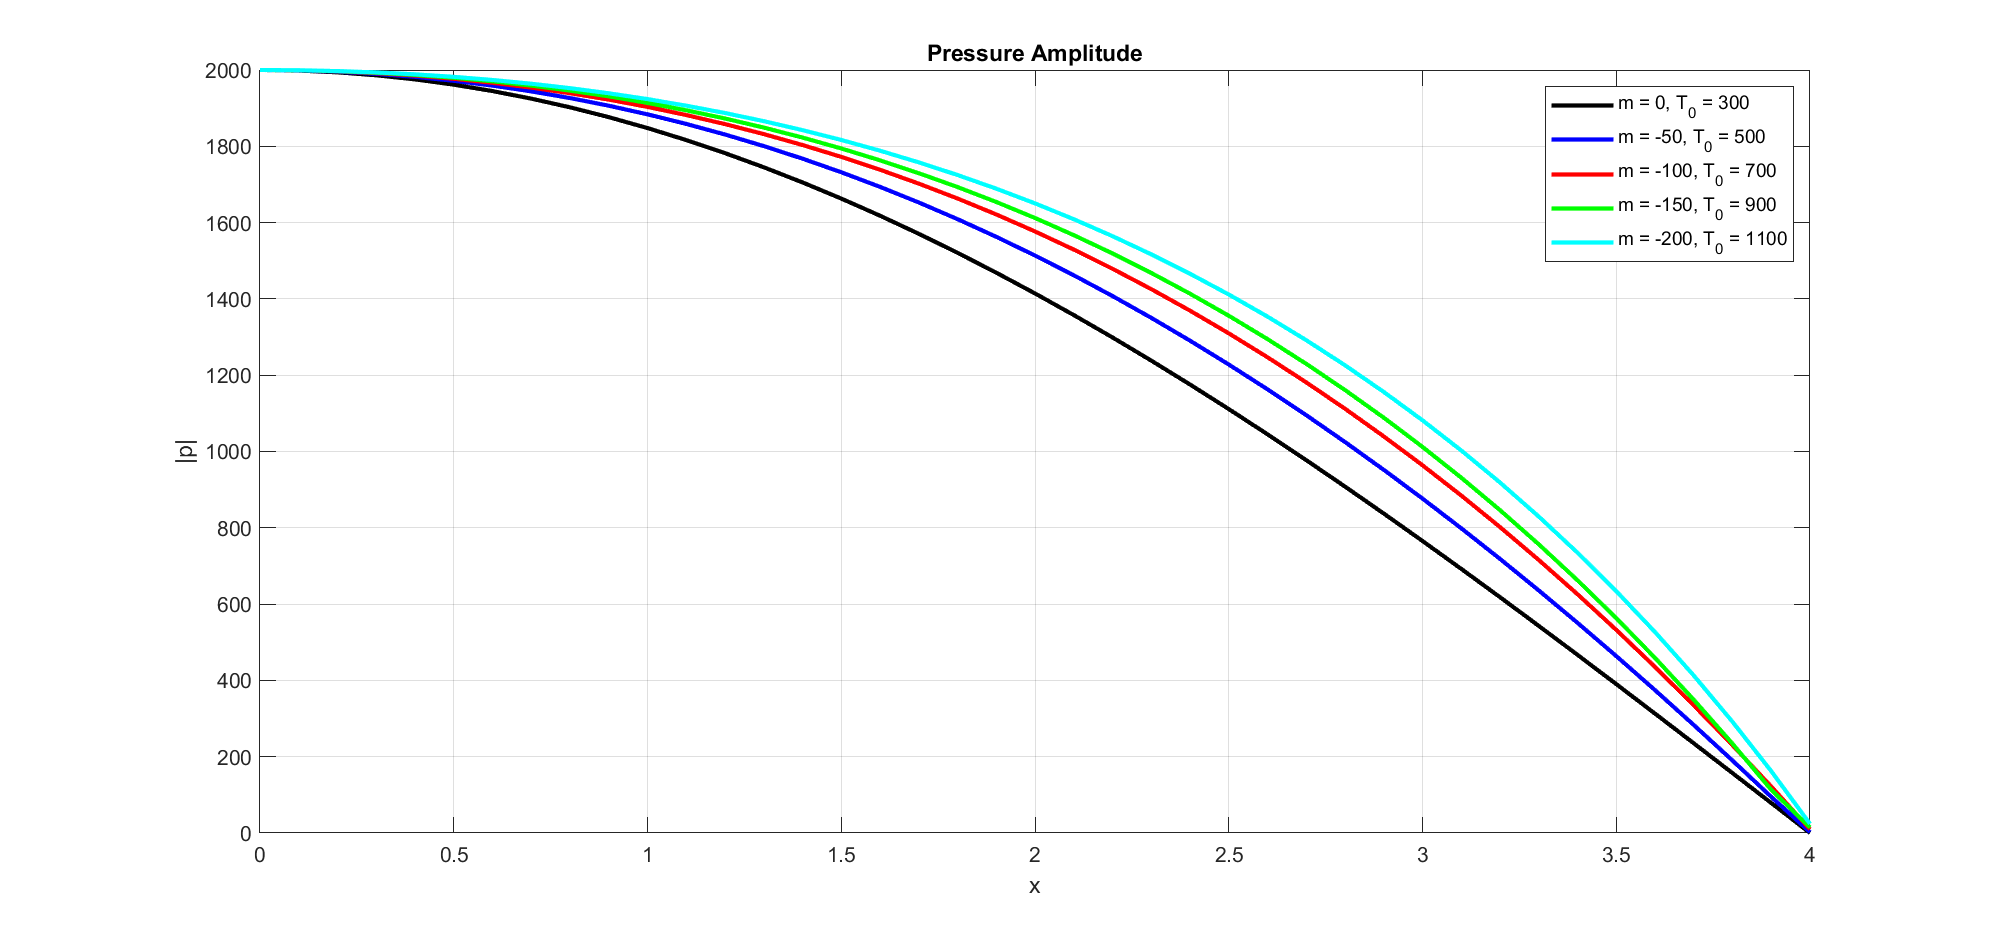
\includegraphics[width=\linewidth]{pvsx1}
    %\caption{Pressure Amplitudes vs x for different linear Temperature Profile}
    \label{fig:pvsx1}
  \end{minipage}
  \hfill
  \begin{minipage}[b]{0.495\linewidth}
    \centering
    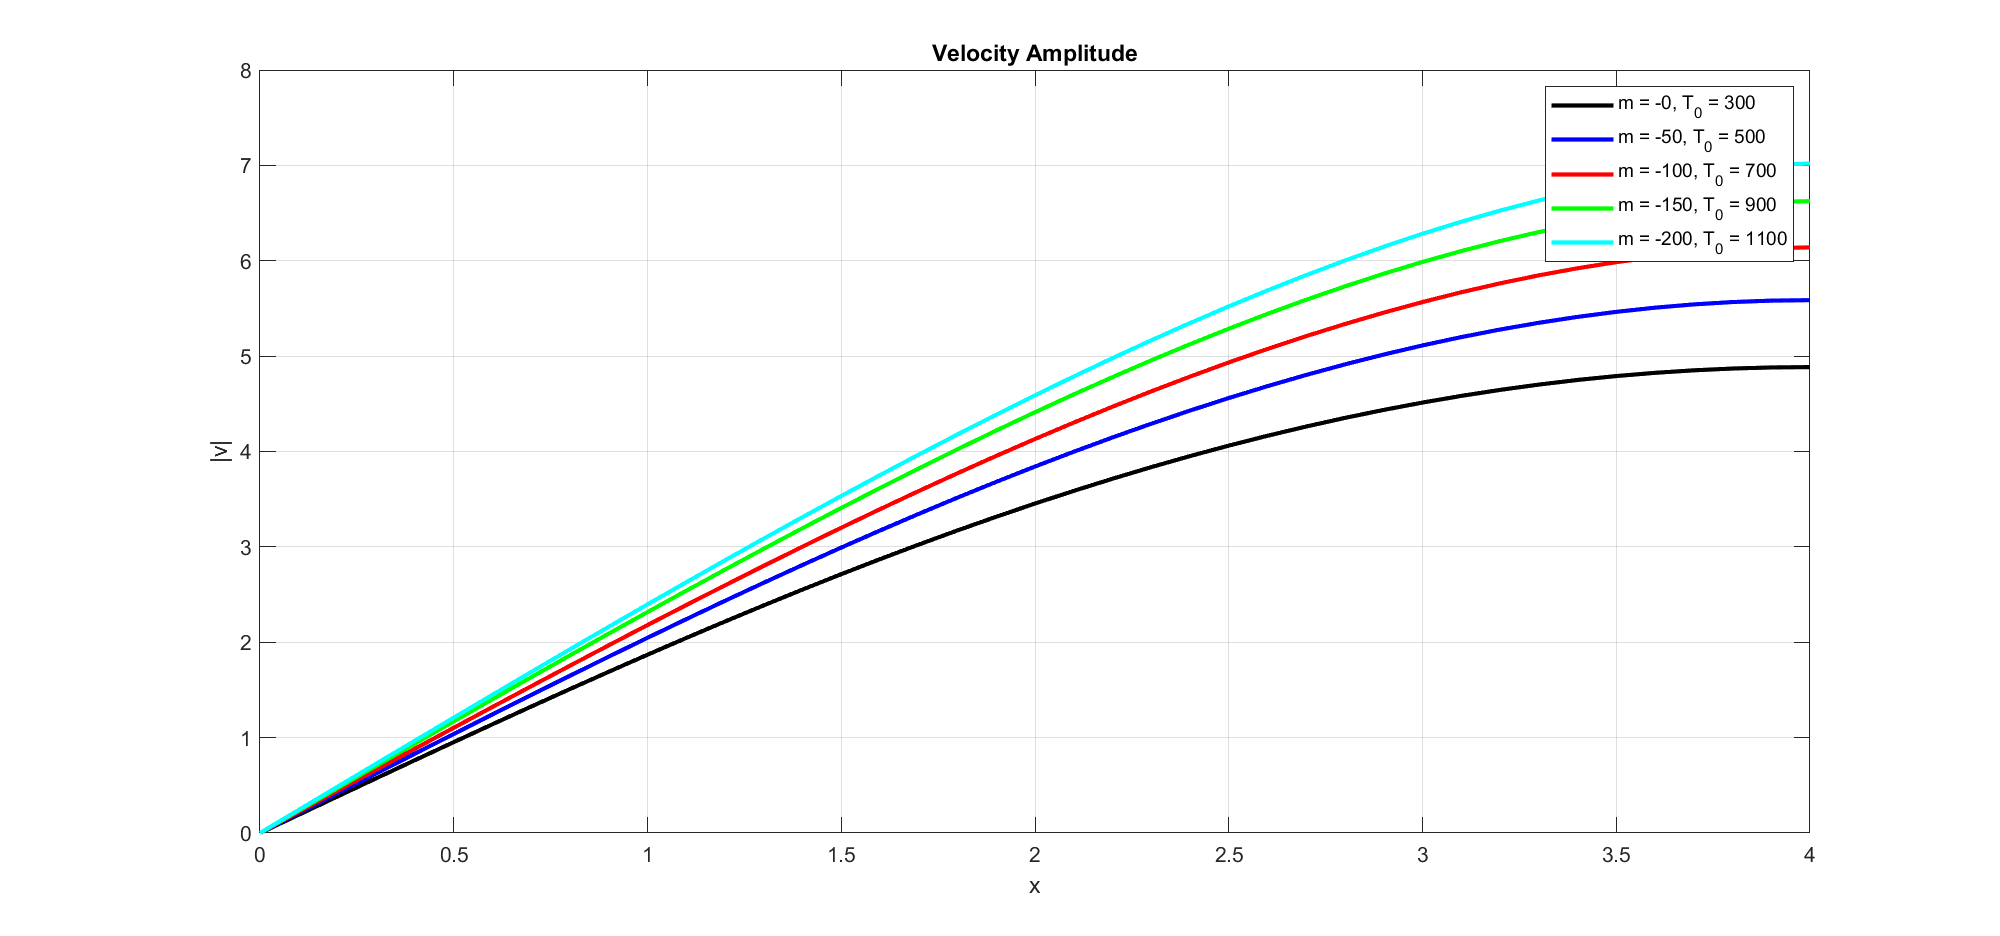
\includegraphics[width=\linewidth]{vvsx1}
    %\caption{Velocity Amplitudes vs x for different linear Temperature Profile}
    \label{fig:vvsx1}
  \end{minipage}
\caption{1st Harmonic / 1st Mode}
\end{figure}

\begin{figure}[H]
  \centering
  \begin{minipage}[b]{0.495\linewidth}
    \centering
    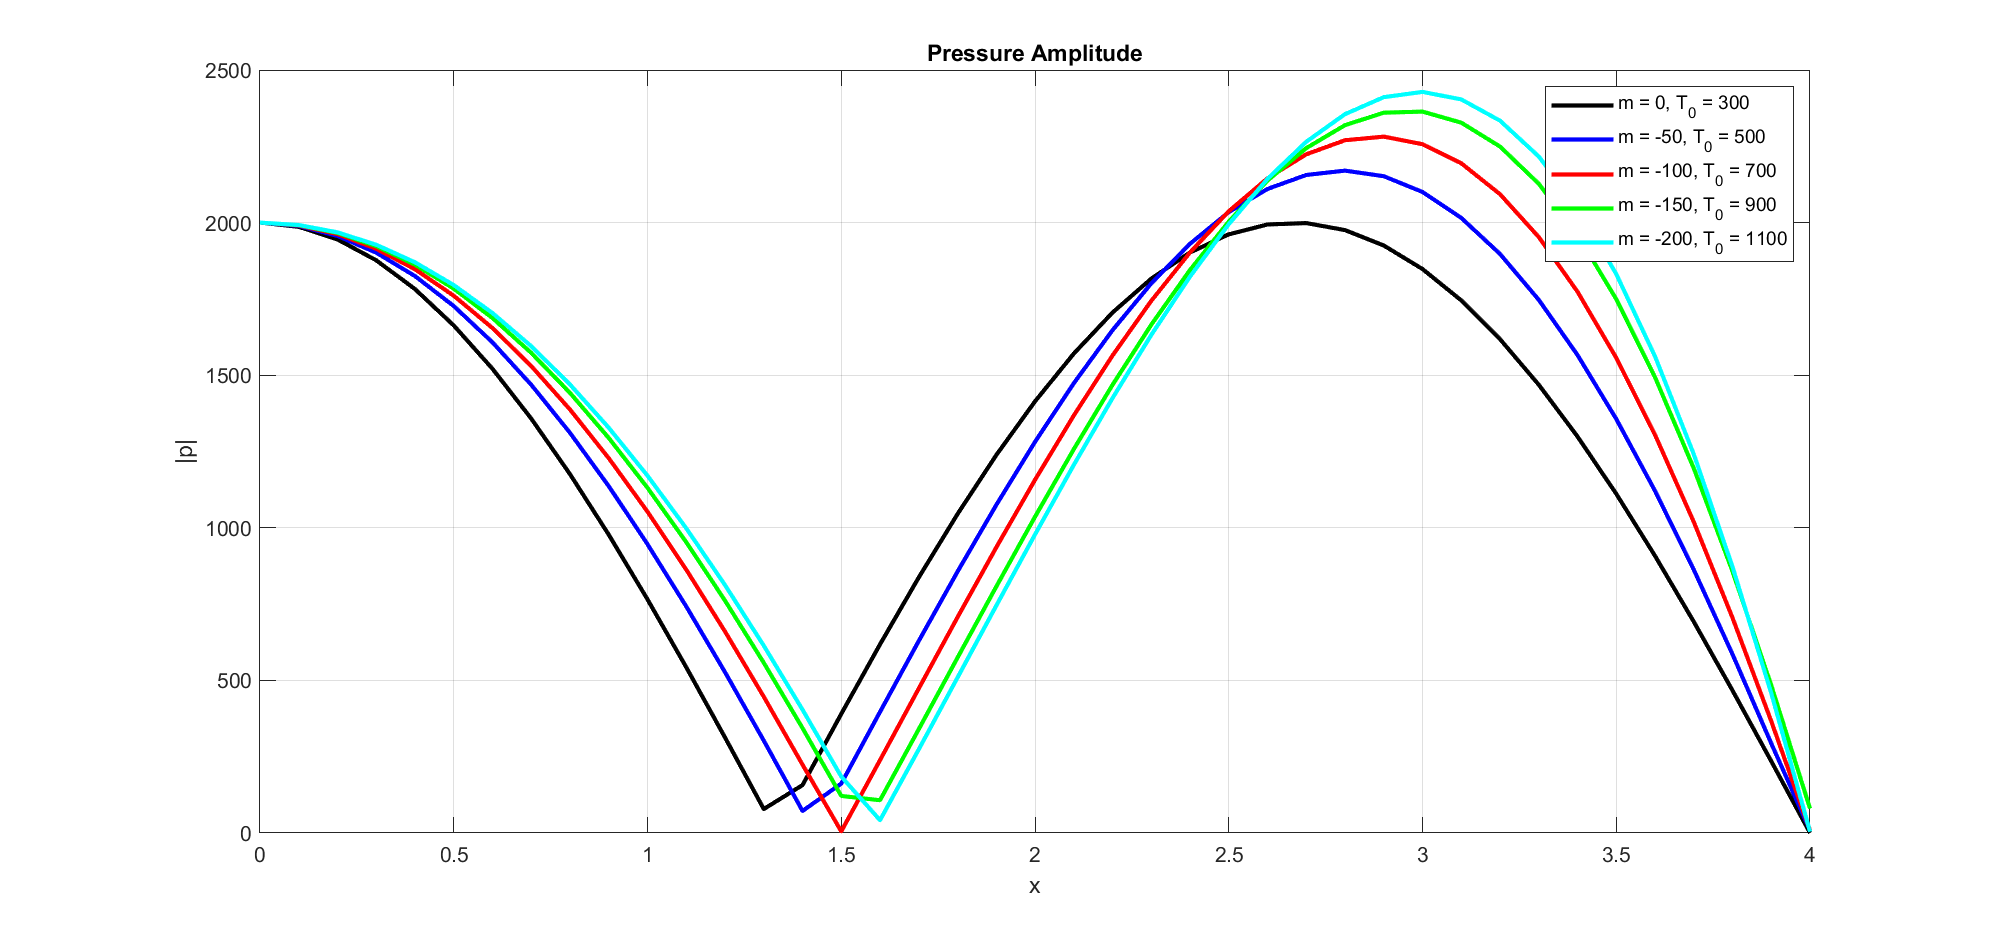
\includegraphics[width=\linewidth]{pvsx2}
    %\caption{Pressure Amplitudes vs x for different linear Temperature Profile}
    \label{fig:pvsx2}
  \end{minipage}
  \hfill
  \begin{minipage}[b]{0.495\linewidth}
    \centering
    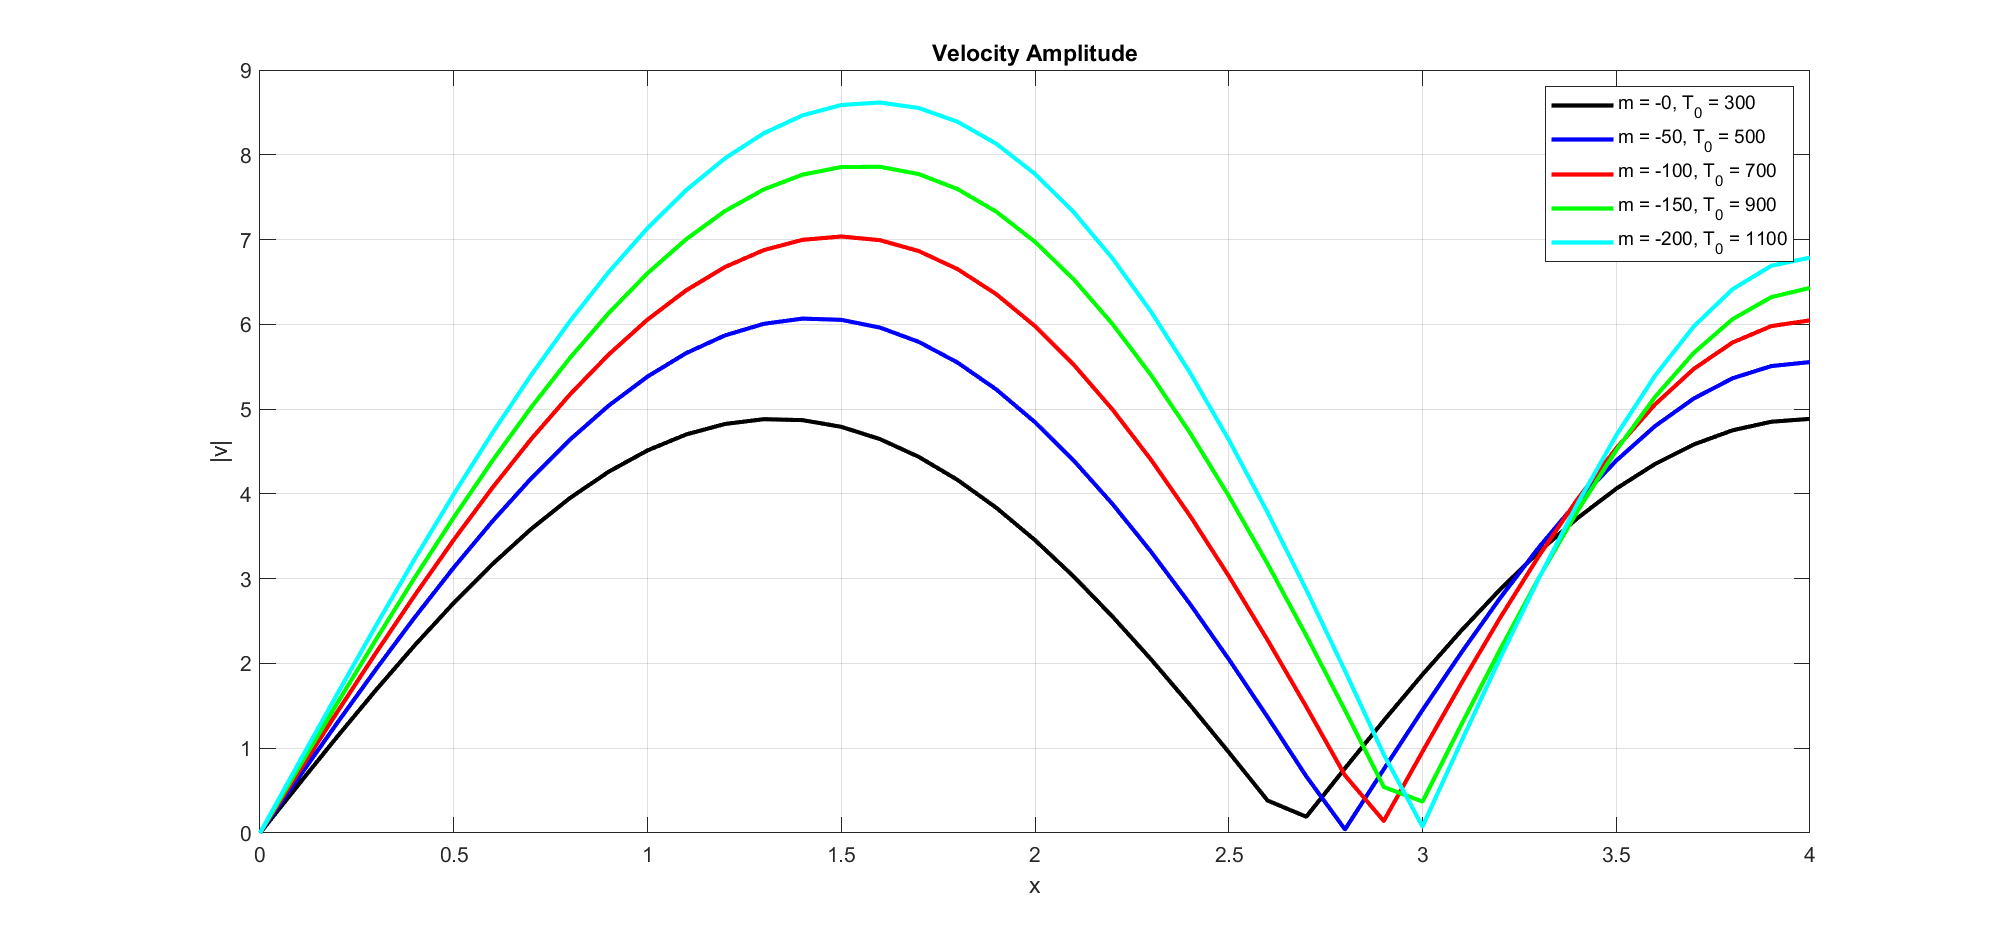
\includegraphics[width=\linewidth]{vvsx2}
    %\caption{Velocity Amplitudes vs x for different linear Temperature Profile}
    \label{fig:vvsx2}
  \end{minipage}
\caption{3rd Harmonic / 2nd Mode}
\end{figure}

\begin{figure}[H]
  \centering
  \begin{minipage}[b]{0.495\linewidth}
    \centering
    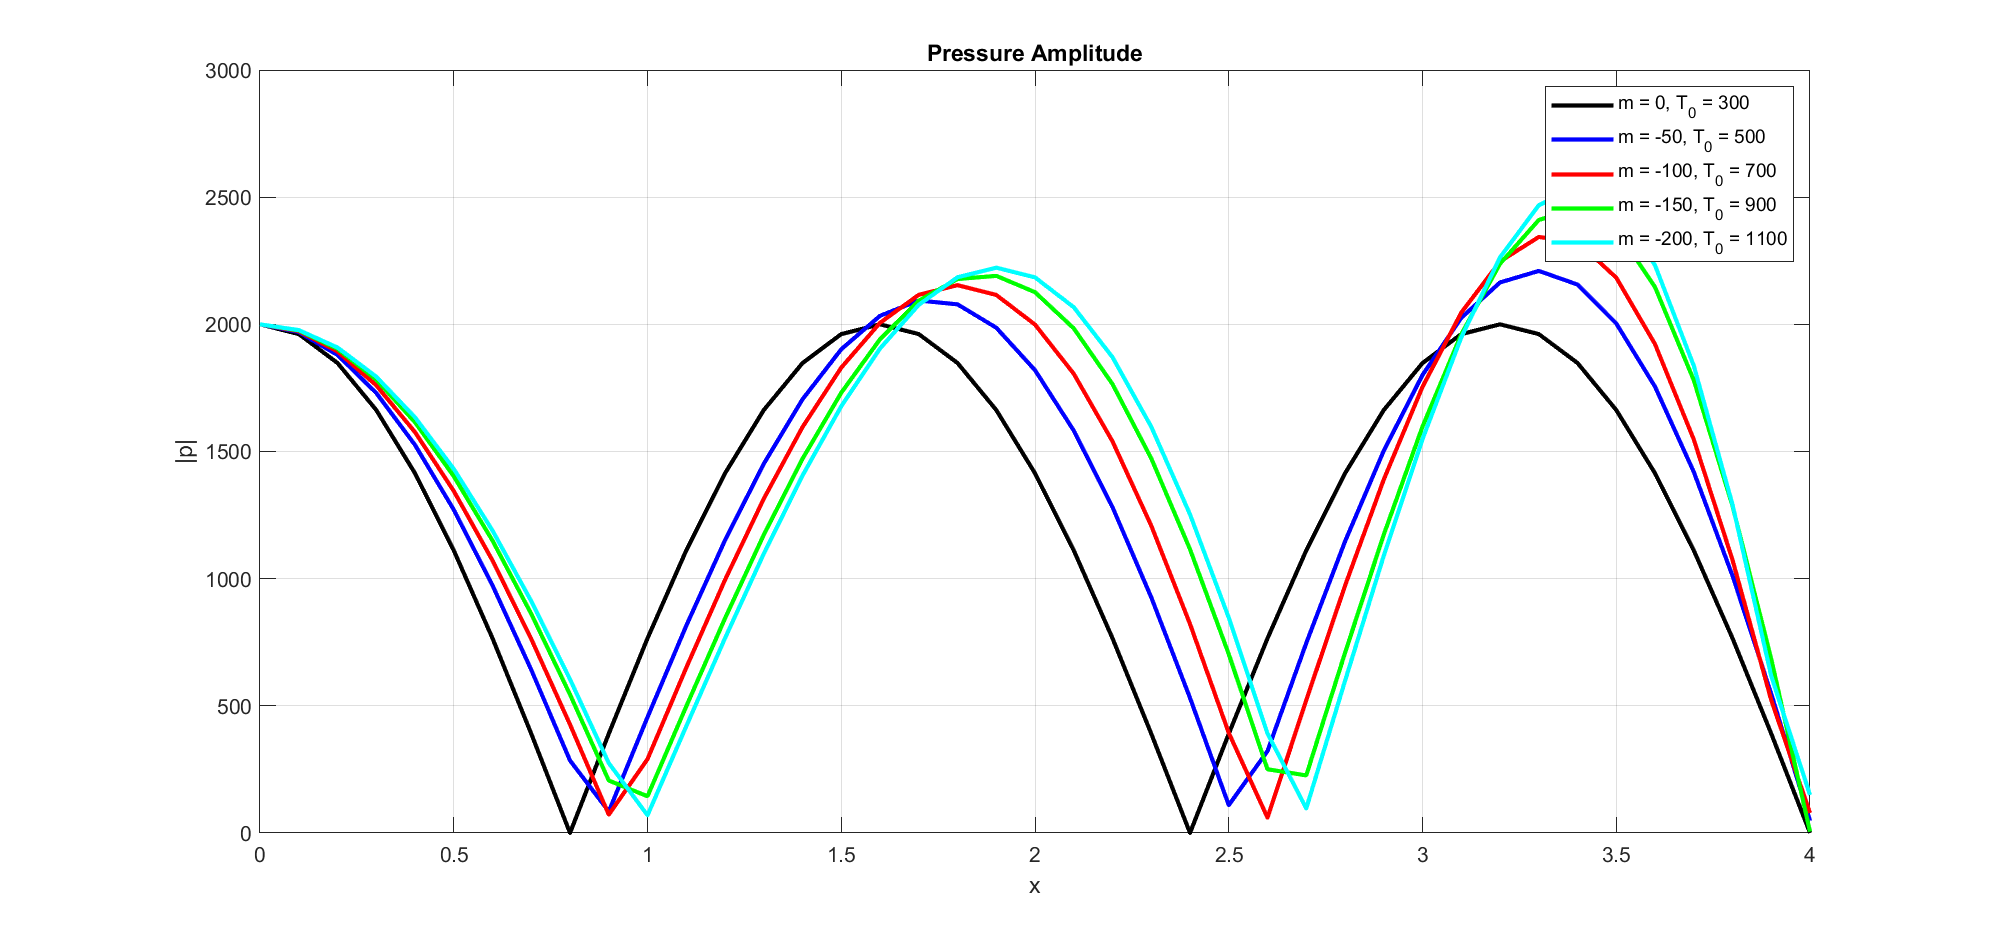
\includegraphics[width=\linewidth]{pvsx3}
    %\caption{Pressure Amplitudes vs x for different linear Temperature Profile}
    \label{fig:pvsx3}
  \end{minipage}
  \hfill
  \begin{minipage}[b]{0.495\linewidth}
    \centering
    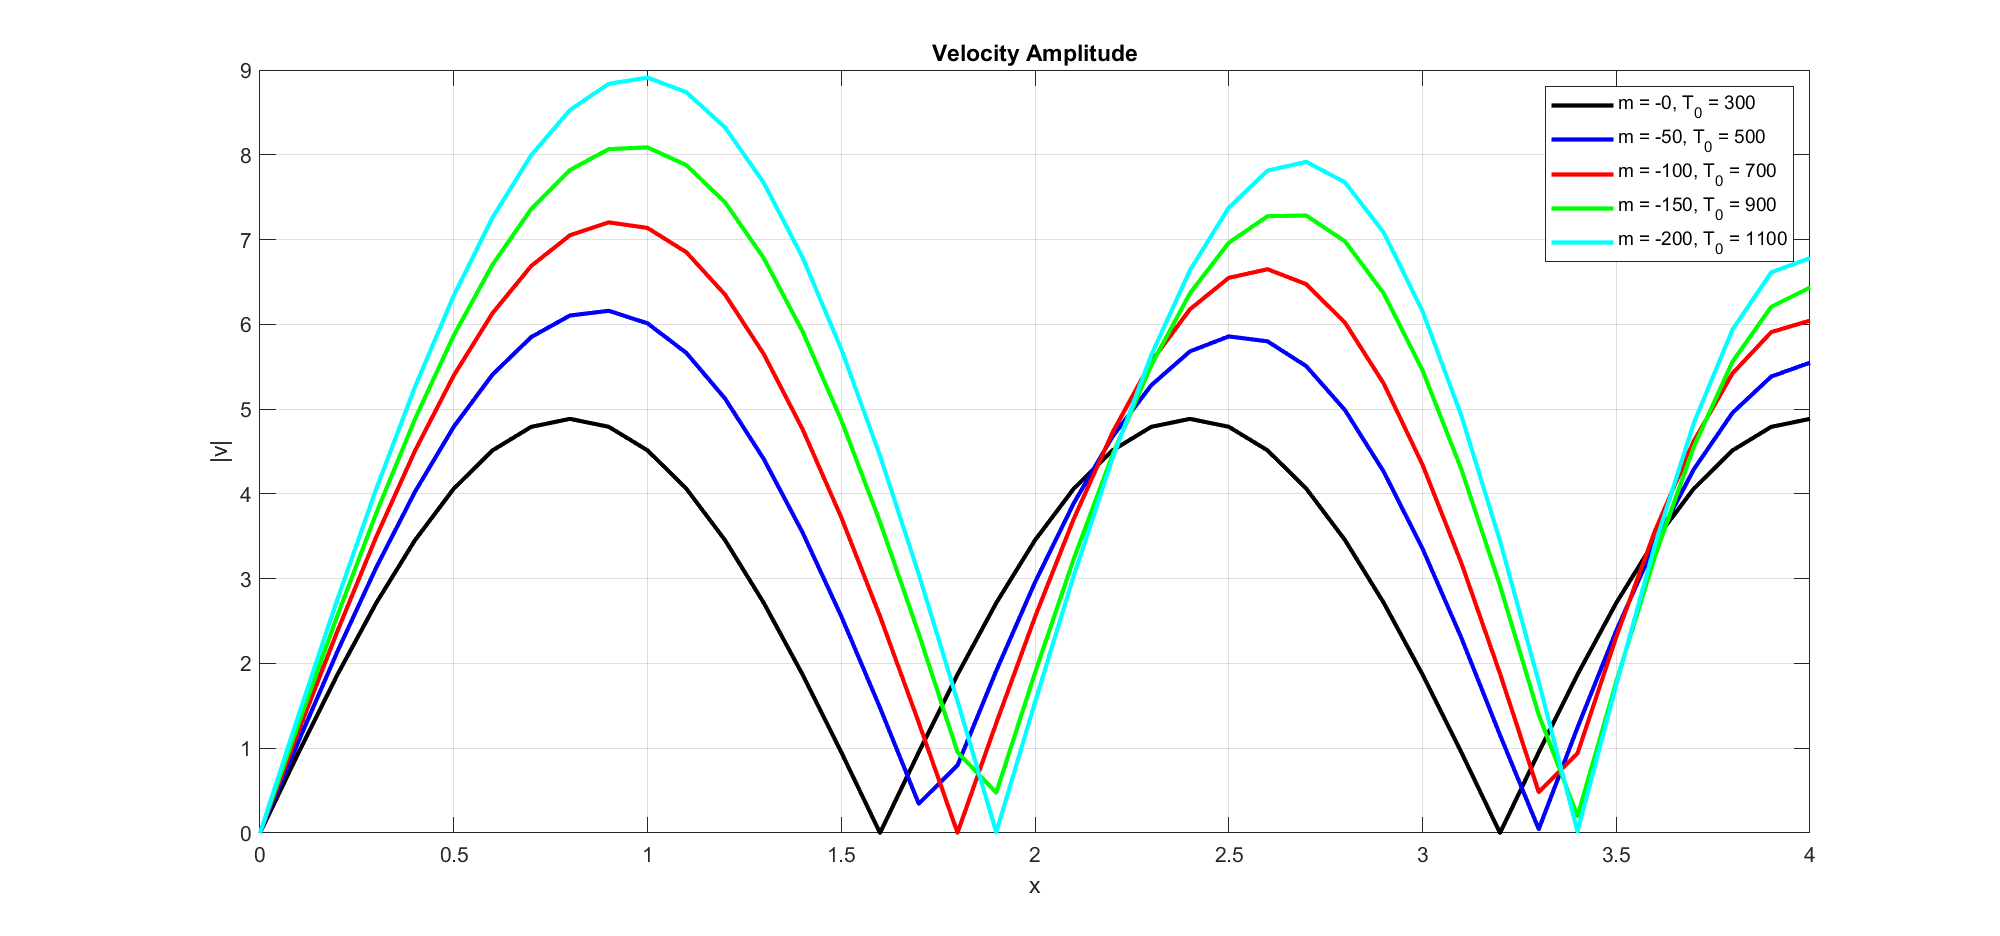
\includegraphics[width=\linewidth]{vvsx3}
    %\caption{Velocity Amplitudes vs x for different linear Temperature Profile}
    \label{fig:vvsx3}
  \end{minipage}
\caption{5th Harmonic / 3rd Mode}
\end{figure}

\begin{figure}[H]
  \centering
  \begin{minipage}[b]{0.495\linewidth}
    \centering
    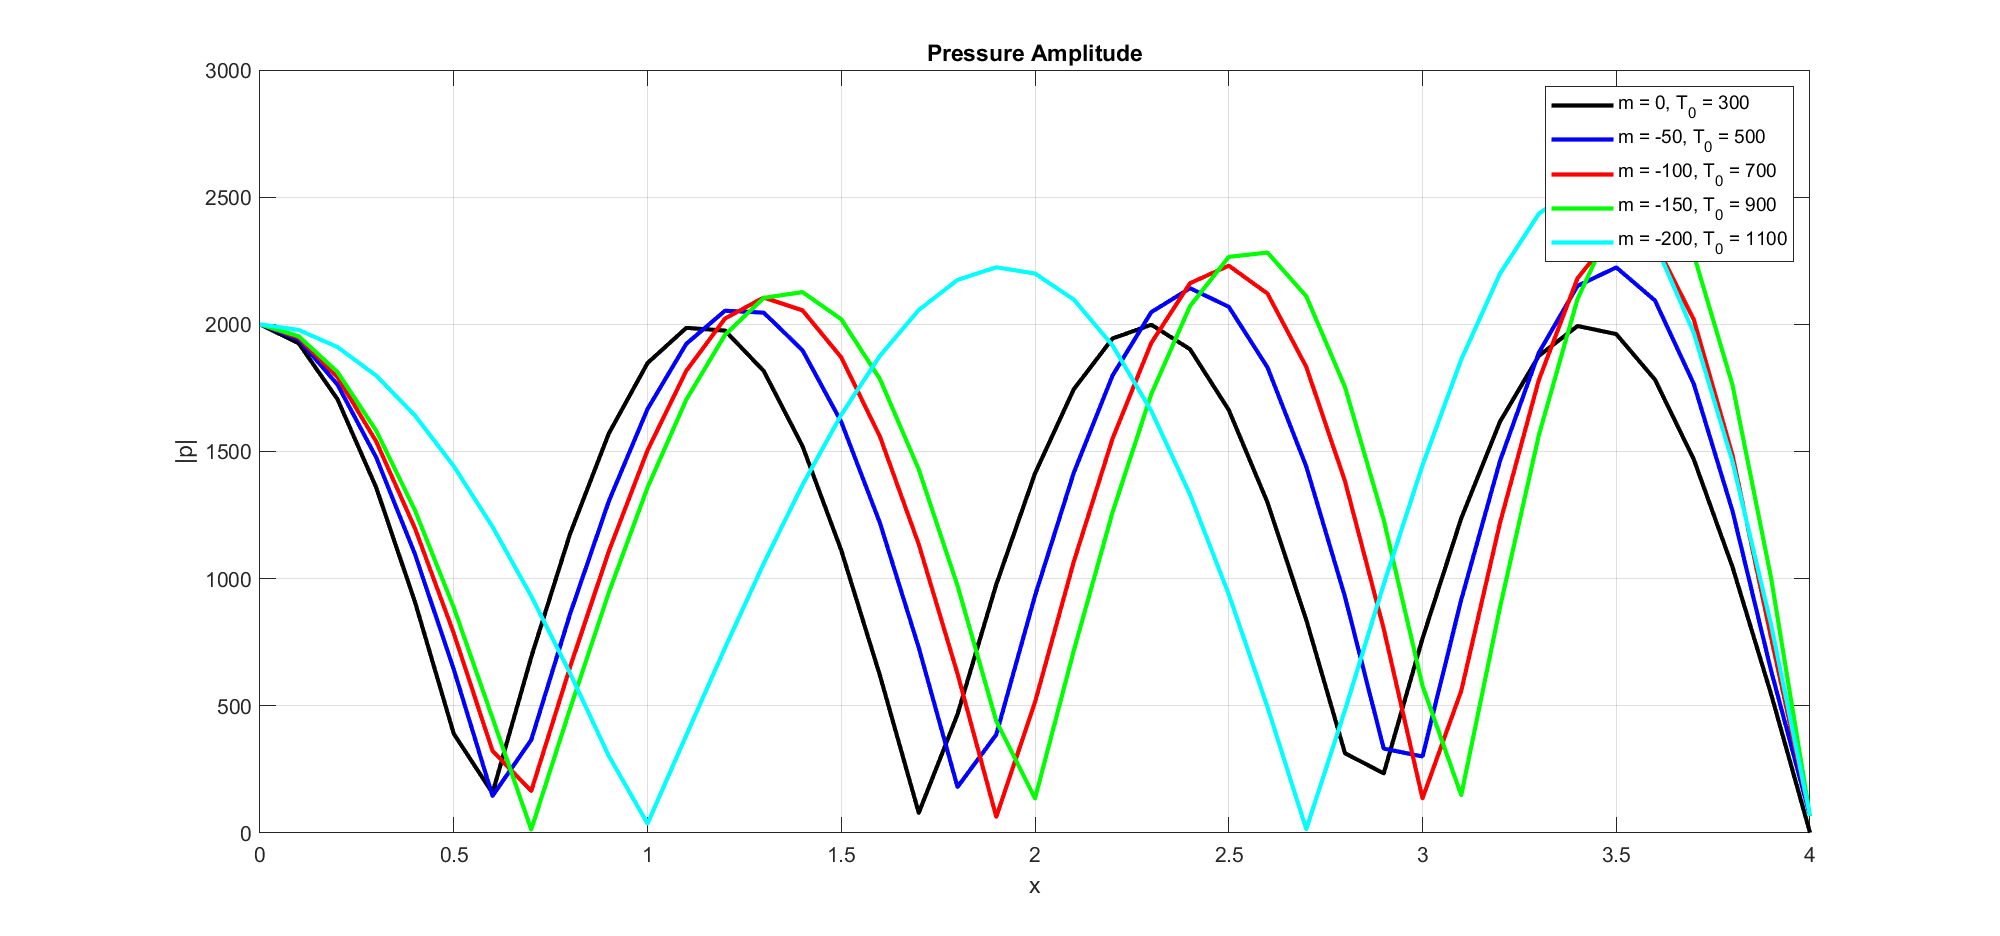
\includegraphics[width=\linewidth]{pvsx4}
    %\caption{Pressure Amplitudes vs x for different linear Temperature Profile}
    \label{fig:pvsx4}
  \end{minipage}
  \hfill
  \begin{minipage}[b]{0.495\linewidth}
    \centering
    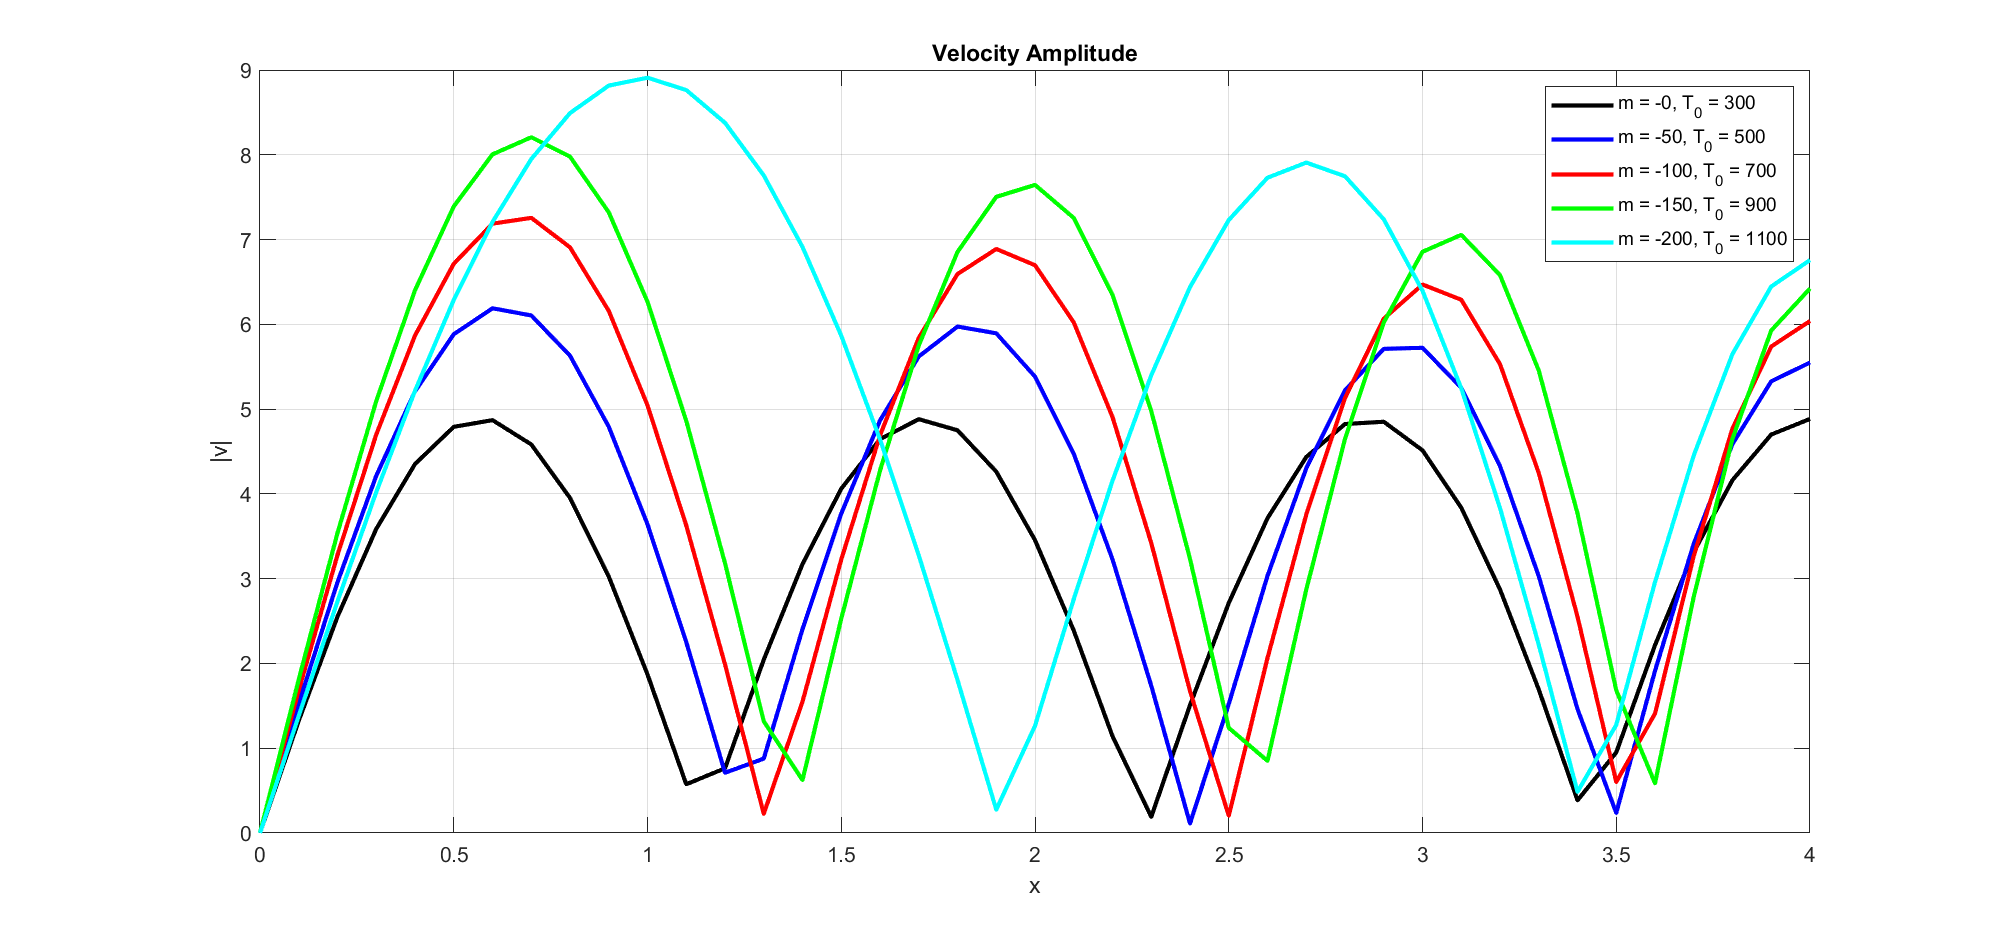
\includegraphics[width=\linewidth]{vvsx4}
    %\caption{Velocity Amplitudes vs x for different linear Temperature Profile}
    \label{fig:vvsx4}
  \end{minipage}
\caption{7th Harmonic / 4th Mode}
\end{figure}

\begin{figure}[H]
  \centering
  \begin{minipage}[b]{0.495\linewidth}
    \centering
    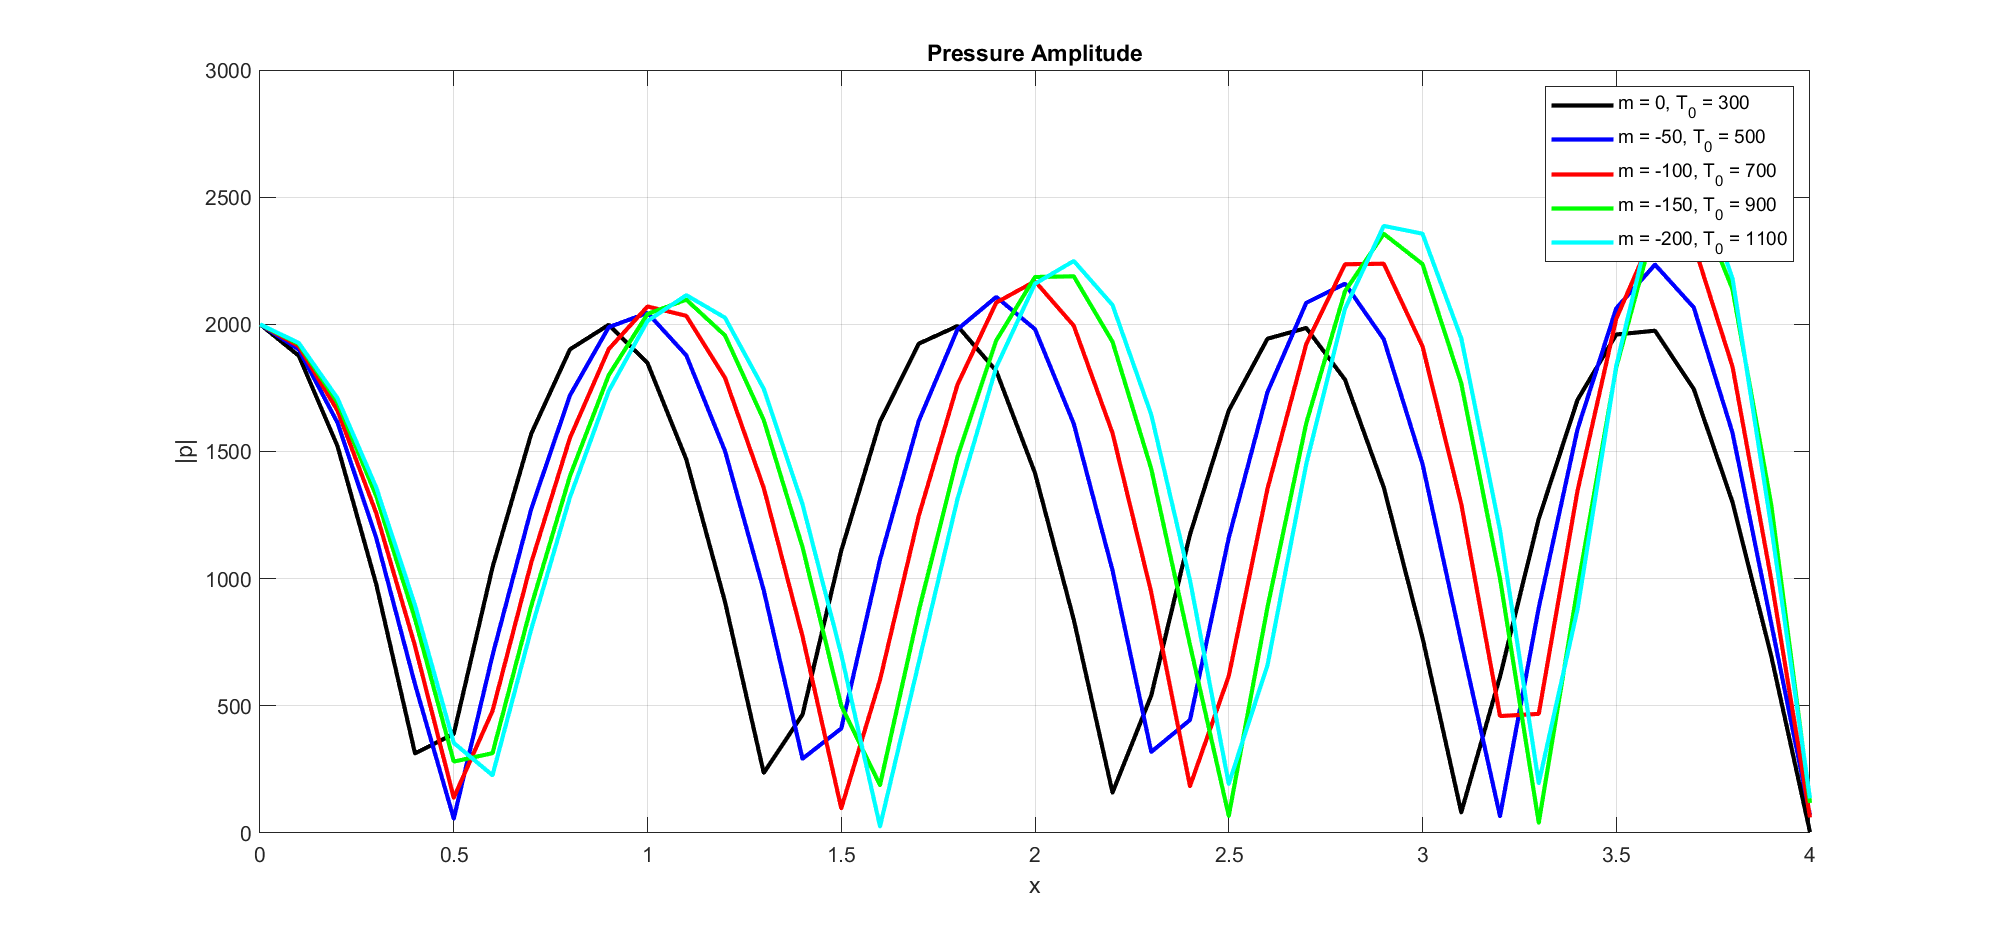
\includegraphics[width=\linewidth]{pvsx5}
    %\caption{Pressure Amplitudes vs x for different linear Temperature Profile}
    \label{fig:pvsx5}
  \end{minipage}
  \hfill
  \begin{minipage}[b]{0.495\linewidth}
    \centering
    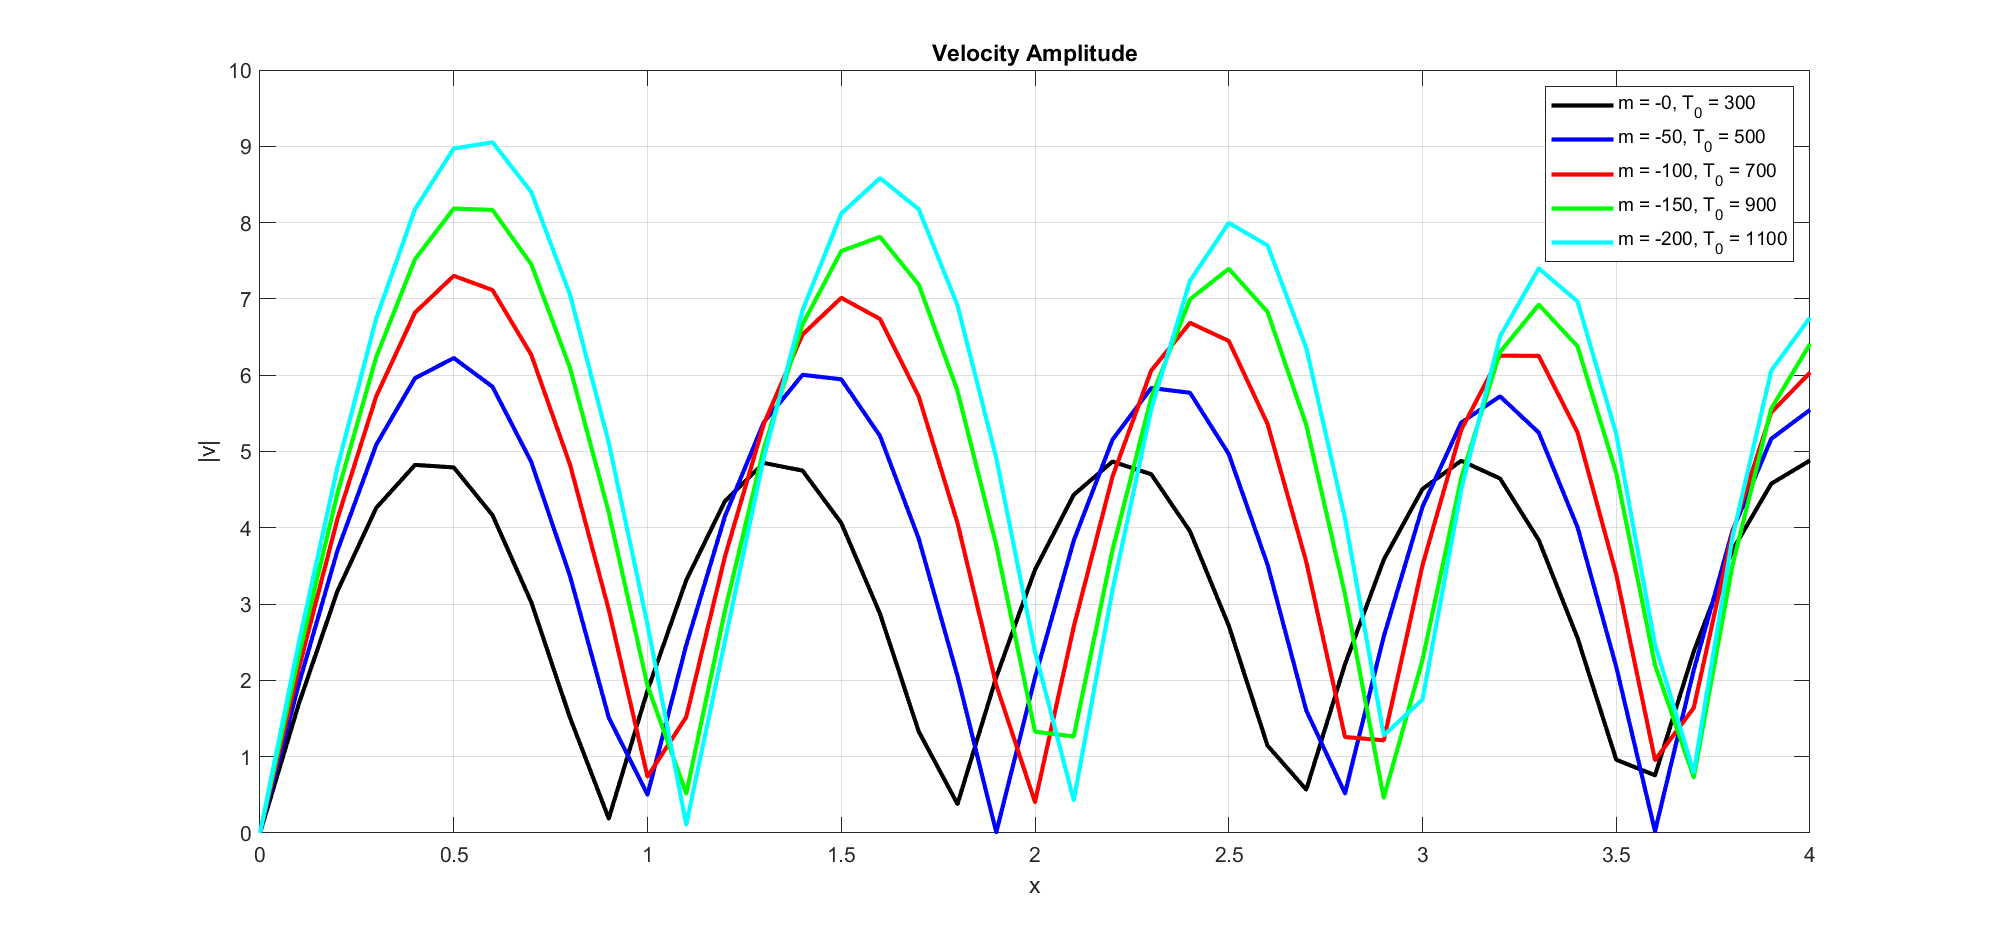
\includegraphics[width=\linewidth]{vvsx5}
    %\caption{Velocity Amplitudes vs x for different linear Temperature Profile}
    \label{fig:vvsx5}
  \end{minipage}
\caption{9th Harmonic / 5th Mode}
\end{figure}

We can have a more closer look at the variation of these variables for one specific mode and temperature distribution below.
\begin{figure}[H]
    \centering
    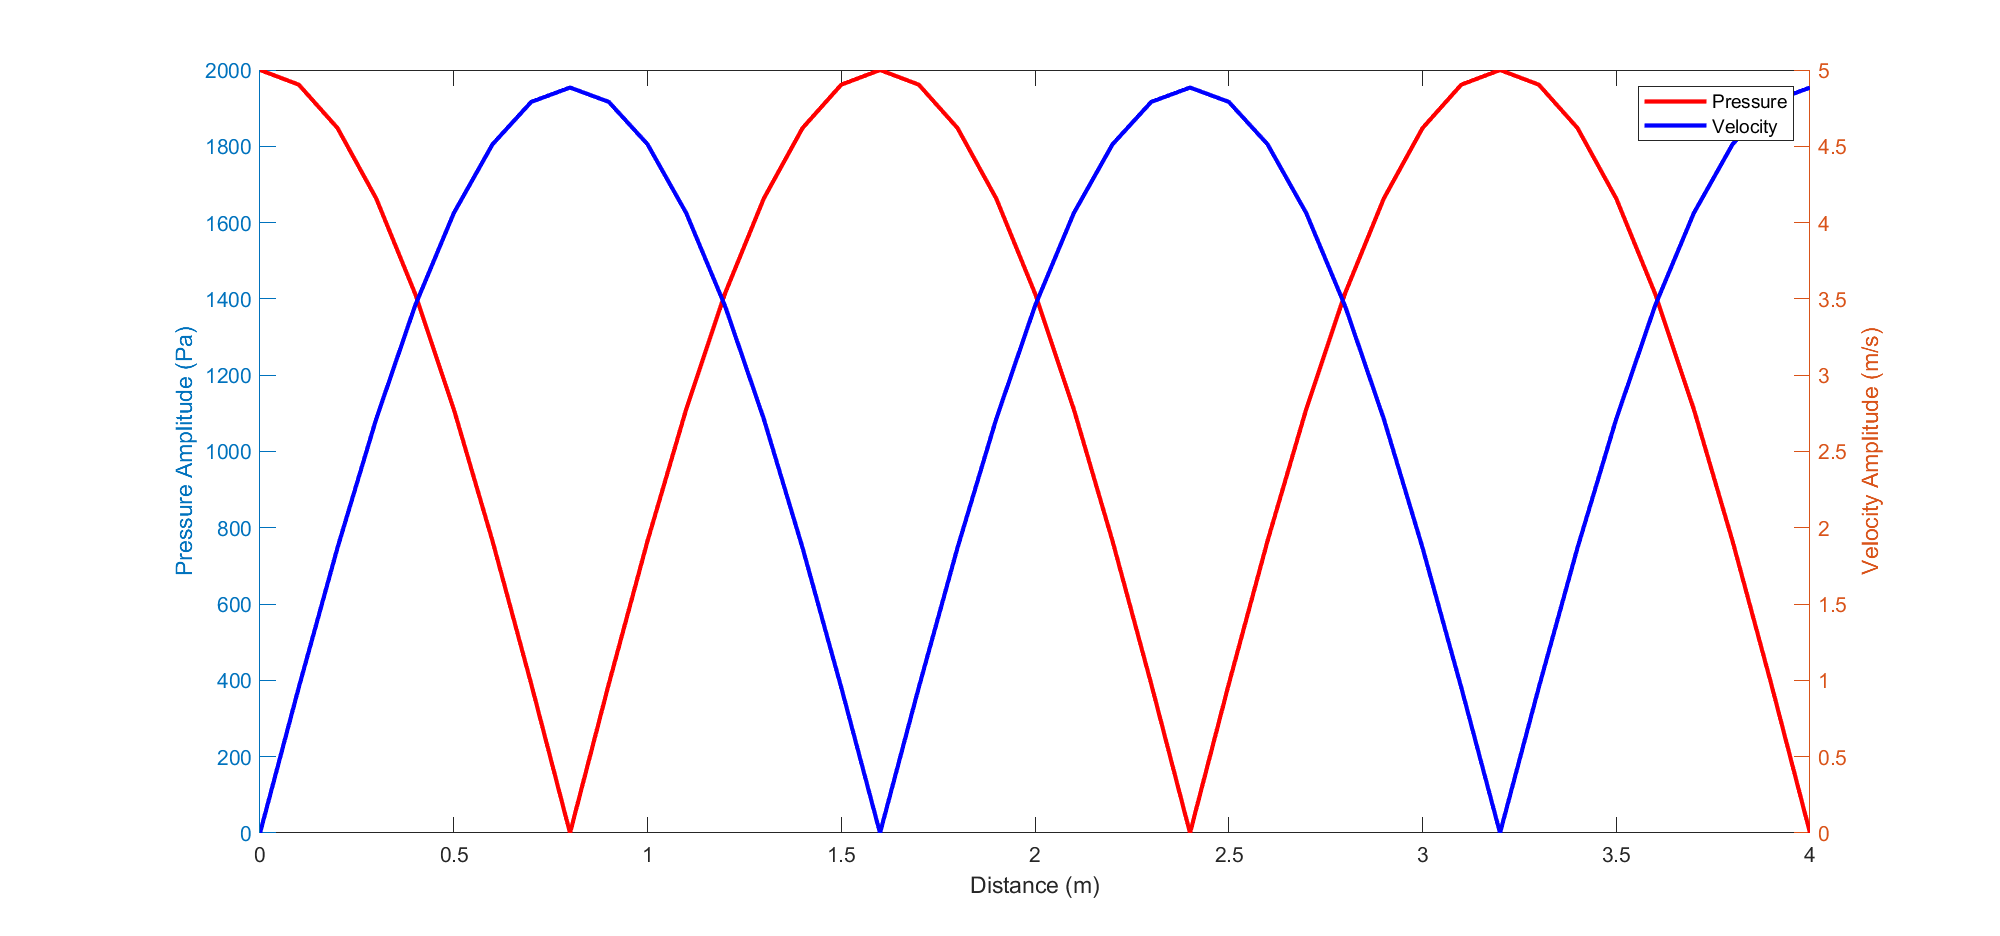
\includegraphics[width=0.8\linewidth]{pv.png}
    \caption{Pressure and Velocity Amplitudes vs x for $\bar{T} = 500 - 50x$ in 5th Harmonic}
    \label{fig:pv3}
\end{figure}

\section{Summary}
 The study begins with the derivation of the wave equation for 1D acoustic fields in ducts with axial temperature gradients. The methodology section outlines the discretization process and the utilization of the Runge-Kutta method for numerical solutions. Results from the study are presented, showcasing various harmonic modes and their corresponding pressure and velocity amplitudes, for each temperature distribution.\\\\
\textbf{Conclusions} 
\begin{itemize}
	\item We can clearly see the nodes and antinodes in each plot, varying according to the different modes.
	\item For all modes shown, we can see that the pressure and velocity amplitude increases with increase in speed of sound, which is due to the higher end temperature and temperature gradient .
	\item The maximum pressure amplitudes are close in magnitude for a particular temperature distribution, for different modes. The same observation can be made for velocity amplitudes.
\end{itemize}

\newpage
\section{Appendix}\label{code}
\begin{lstlisting}
% Initial conditions
y1_0 = 2000;
y2_0 = 0;

% Spatial domain
L = 4;
N = 41;
x = linspace(0, L, N);
dx = x(2) - x(1);

%define system parameters
n = 5;
L = 4;
gamma = 1.4;
R = 287;
Pbar = 101532;

p=[];u=[];%initialising arrays for plotting 
omega = zeros(1,4);
    
%looping for different linear temperature profiles
for j=1:5
    %different linear temperature profiles
    m = 50-j*50;
    T0 = 100 + j*200;

    pend=1000000000;
    for ij = 1:N
        w = 2*pi*(n*sqrt(gamma*R*(T0 + m*x(ij))))/(4*L);

        % Preallocate arrays
        y1 = zeros(1, N);
        y2 = zeros(1, N);
        uu = zeros(1, N);
    
        % Set initial values
        y1(1) = y1_0;
        y2(1) = y2_0;
        uu(1) = -((4*L*sqrt(R*T0))/(2*pi*n*Pbar*sqrt(1.4)))*y2(1);

        % Fourth-order Runge-Kutta method
        for i = 1:N-1
            [k1, l1] = equations(x(i), y1(i), y2(i),m,T0,n,L,gamma,R,w);
            [k2, l2] = equations(x(i) + 0.5*dx, y1(i) + 0.5*dx*k1, y2(i) + 0.5*dx*l1,m,T0,n,L,gamma,R,w);
            [k3, l3] = equations(x(i) + 0.5*dx, y1(i) + 0.5*dx*k2, y2(i) + 0.5*dx*l2,m,T0,n,L,gamma,R,w);
            [k4, l4] = equations(x(i) + dx, y1(i) + dx*k3, y2(i) + dx*l3,m,T0,n,L,gamma,R,w);
        
            y1(i+1) = y1(i) + (dx/6) * (k1 + 2*k2 + 2*k3 + k4);
            y2(i+1) = y2(i) + (dx/6) * (l1 + 2*l2 + 2*l3 + l4);
    
            uu(i+1) = -(((R*(T0 + m*i*dx)))/(w*Pbar))*y2(i+1);
        end
        if abs(y1(41))<pend
            Y1 = y1;
            Y2 = y2;
            U = uu;
            pend = abs(Y1(41));
            omega(j) = w;
        end
    end    
    p = [p Y1];
    u = [u U];
end

omega/(2*pi)

% Plotting solutions for system of equations
figure(1);
axis equal
plot(x, Y1, 'b', x, Y2, 'r');
title('Solution of Coupled ODEs');
xlabel('x');
ylabel('y1, y2');
legend('y1', 'y2');
grid on;

%plot of pressure amplitudes for different linear axial temperature profiles
figure2=figure(2);
plot(x, abs(p(1:41)), 'k',x, abs(p(42:82)), 'b',x, abs(p(83:123)), 'r',x, abs(p(124:164)), 'g',x, abs(p(165:205)), 'c','linewidth',2);
title('Pressure Amplitude');
xlabel('x');
ylabel('|p|');
legend('m = -50, T_0 = 500','m = -100, T_0 = 700','m = -150, T_0 = 900','m = -200, T_0 = 1100');
grid on;
saveas(figure2,'pvsx3.png')

%plot of velocity amplitudes for different linear axial temperature profiles
figure3=figure(3);
plot(x, abs(u(1:41)), 'k',x, abs(u(42:82)), 'b',x, abs(u(83:123)), 'r',x, abs(u(124:164)), 'g',x, abs(u(165:205)), 'c','linewidth',2);
title('Velocity Amplitude');
xlabel('x');
ylabel('|v|');
legend('m = -50, T_0 = 500','m = -100, T_0 = 700','m = -150, T_0 = 900','m = -200, T_0 = 1100');
grid on;
saveas(figure3,'vvsx3.png')

%plot of comparison of pressure and velocity amplitudes
figure4=figure(4);
yyaxis left
plot(x, abs(p(1:41)), 'r','linewidth',2);
xlabel('Distance (m)');
ylabel('Pressure Amplitude (Pa)');
yyaxis right
plot(x, abs(u(1:41)), 'b','linewidth',2);
ylabel('Velocity Amplitude (m/s)');
legend('Pressure', 'Velocity');
saveas(figure4,'pv3.png') 

% Define the functions f1(x, y1, y2) and f2(x, y1, y2)
function [dy1_dx, dy2_dx] = equations(x, y1, y2,m,T0,n,L,gamma,R,w)
    %define temperature profile
    Tbar = T0 + m*x;
    
    % Define the system of equations
    dy1_dx = y2;
    dy2_dx = -((w^2)/(gamma*R*Tbar)) * y1 - (m/Tbar) * y2;
end
\end{lstlisting}

\section{Bibliography}
\begin{thebibliography}{99}

\bibitem{refpaper}
An exact solution for one-dimensional acoustic fields in ducts with an axial temperature gradient\\ \url{https://www.sciencedirect.com/science/article/pii/S0022460X85703239}
\end{thebibliography}


\end{document}